% Author: Bernard Lampe

% Use the IEEE classes
\documentclass[journal]{IEEEtran}

% Packages
\usepackage[cmex10]{amsmath}
\usepackage{url}
\usepackage{cite}
\usepackage{graphicx}
\usepackage{subfig}
\usepackage{float}
\usepackage{morefloats}

% Correct bad hyphenation here
\hyphenation{op-tical net-works semi-conduc-tor}
\DeclareMathOperator*{\argmax}{arg\,max}
\DeclareMathOperator*{\argmin}{arg\,min}

% Start document
\begin{document}

% Paper title
\title{Kernel Discriminant Functions for Classification}

% Author
\author{Bernard~Lampe,~\IEEEmembership{Member,~IEEE}}

% The paper headers
\markboth{Kernel Discriminant Functions for Classification}
{Shell \MakeLowercase{\Lampe}: Kernel Discriminant Functions for Classification}

\maketitle

\begin{abstract}
In this study we investigate the effectiveness of augmenting support vector machine (SVM) and Fisher linear discriminant analysis (FLDA) classifiers using known kernel methods. Strictly speaking Fishers is a data reduction technique, and we extend it to build a classifier. The extension was done in two ways using Euclidean and Mahalanobis distance metrics. We test the three well known kernels of polynomial, tangent hyperbolic sigmoid and radial basis function (RBF). We judge the effectiveness of these kernels and classifiers on a five class problem based on a biased coin which implies binomial class distributions of differing means and variances.
\end{abstract}

% Keywords
\begin{IEEEkeywords}
Multi-class Classification, Kernel Fisher Linear Discriminant Analysis, Kernel Support Vector Machine, KFLDA, KSVM
\end{IEEEkeywords}

% Introduction with drop letter and first word capitalized.
\section{Introduction}

\IEEEPARstart{F}{ishers} linear discriminant analysis (FLDA) and support vector machines (SVM) aim to find an optimal linear hyperplane which will provide the best discriminating power between labeled class instances. These supervised training methods perform very well when the classes can be linearly separated. However, many real-world problems have non-linear or inseparable data when considering data in the original feature space. To overcome these non-linearities we could try to use more complicated parametric models to approximate the class conditional probabilities and then construct a Bayes classifier. This method gives us little idea on what model to choose or how to extend an analytical form which will remain computationally tractable. We could also attempt to estimate the class conditionals using non-parametric methods. However, this approach requires an exponential number of data samples from each class as the dimensionality of the feature space is increased. A more effective approach is to make the data linearly separable by mapping the data to a higher dimension feature space \(F\) via non-linear mapping \(\Phi(\vec{x^n})\). If \(F\) is of a very high dimensionality or infinitely dimensional, the mapping will be impossible to compute. To overcome this limitation a kernel trick is used to compute dot products \(\Phi(\vec{x^i})\cdot\Phi(\vec{x^j})\) between vectors in the feature space \(F\) without explicitly computing the vectors themselves. This is accomplished via Mercer kernels\cite{mercer}\cite{mika}. A discussion of Mercers theorem, FLDA and SVM is beyond the scope of this report and there are many very thorough references \cite{alpaydin}\cite{chang2}\cite{mercer}.

% Describe Experiments
\section{Training Data and Test Sample Generation}
\par In this study the training data was simulated by flipping a hypothetical coin \(d=100\) times. The training observations were labeled with the target value \(t = i\) which indexes the class \(C_i\). We consider the five class problem and the data was generated by flipping five different, biased coins. The biases are in the set \(\Theta = \{0.1, 0.2, 0.3, 0.4, 0.5\}\). The data pool consists of 3000 samples each of 100 flips such that \(\Delta_i = \{\vec{x}_i^j\}_{j=1}^{200i}\) and \(\Delta = \cup_{i=1}^5{\Delta_i}\). The n-th training sample of \(\Delta\) is a tuple of the sample vector and target value \((\vec{x}^n, t^n)\). For all training runs, the data was partitioned into two equal sized groups. Half of the training samples were used to train the classifier. The other half were used as new test observations.

\section{Kernel Function Formulations}
\par There are many Mercer kernels which can be used to perform the kernel trick. To speed computation we compute the Gram matrix which is essentially applying the kernel trick to all pairs of training observations in \(\Delta\). We implemented the polynomial kernel as in equation \ref{eq:polykernel}, the tangent hyperbolic sigmoid kernel as in equation \ref{eq:sigkernel} and the radial basis function (RBF) kernel as in equation \ref{eq:rbfkernel}. Each KFLDA and KSVM method we implemented in this study applied the kernel to the data and not the feature vectors.

\begin{equation}
\label{eq:polykernel}
K(\vec{x_i}, \vec{x_j}) = (\gamma\vec{x_i}^T\vec{x_j} + c)^d
\end{equation}

\begin{equation}
\label{eq:sigkernel}
K(\vec{x_i}, \vec{x_j}) = \tanh(\gamma\vec{x_i}^T\vec{x_j} + c)
\end{equation}

\begin{equation}
\label{eq:rbfkernel}
K(\vec{x_i}, \vec{x_j}) = \exp{\left( -\frac{\left\| \vec{x_i} - \vec{x_j}\right\|}{2\sigma^2}\right)}
\end{equation}

\section{KFLDA Classification Distance Metrics}
\par To extend the kernel Fishers linear discriminant analysis (KFLDA) from a data reduction method to a classifier, we start by computing the KFLDA feature vectors as described in the references by Mika, Max, Baudat or Park \cite{mika}\cite{max}\cite{baudat}\cite{park}. We have five classes therefore the subspace has four feature vectors and dimensions. We compute the projected means, \(\vec{\mu_i}\) and covariances \(\vec{\Sigma_i}\) for each class in the subspace. After we have the feature vectors, projected class means and projected covariances, we can dismiss the original training data. Finally to classify new samples, we project new sample into the subspace made up of these four feature vectors and compute the distances to each class using the means and covariances. We derive the distance metric by starting with the optimal Bayes classifier as in equation \ref{eq:jointprob}. For computational tractability we then assume the class conditionals are effectively modeled by a Gaussian. This assumption is not unfounded due to the binomial nature of the random variable. If we combine equations \ref{eq:jointprob} and \ref{eq:assumegauss} then we arrive at equation \ref{eq:maha}. We refer to this distance throughout the remaining portion of this paper as the Mahalanobis distance though strictly speaking, this distance is closer related to the Bhattacharyya distance \cite[p.~166]{chang1}.

\begin{equation}
\label{eq:jointprob}
C^* = \argmax_{C_i}\{log(p(\vec{x}|C_i)) + log(p(C_i))\}
\end{equation}

\begin{equation}
\label{eq:assumegauss}
p(\vec{x}|C_i) = \frac{1}{(2\pi)^{\frac{d}{2}}} \left| \Sigma_i \right|\exp{\left\{-\frac{1}{2}(\vec{x}-\vec{\mu_i}^T\Sigma_i^{-1}(\vec{x}-\vec{\mu_i})\right\}}
\end{equation}

\begin{align}
C^* = \argmax_{C_i}\{ &-\frac{1}{2} log(\left|\Sigma_i\right|) - \frac{1}{2}(\vec{x} - \vec{\mu_i})^T\Sigma_i^{-1}(\vec{x}-\vec{\mu_i}) \label{eq:maha} \\
& {} + log(p(C_i)) \nonumber \}
\end{align}

\par To compute the Mahalanobis distance from a new observation \(\vec{x}\) to each class \(C_i\) using the formula in \ref{eq:maha}, we need to estimate the class priors, means and covariances using the maximum likelihood estimators in equations \ref{eq:priorest}, \ref{eq:meanest} and \ref{eq:covest}. In each of the equations below, \(W\) is the \(3000x4\) matrix consisting of feature vectors computed via KFDLA and \(W_n^T\) is a \(4x1\) vector from a single row in W.

\begin{equation}
\label{eq:indicator}
N_i = \sum_{n=1}^{N}{r_i^n}, \text{    where     }  r_i^n =
\begin{cases}
 1 ,& \text{    if    } \vec{x}^n \in C_i \\
 0         ,& \text{otherwise}
\end{cases}
\end{equation}

\begin{equation}
\label{eq:priorest}
p(C_i) \approx \hat{p}(C_i) = \frac{N_i}{N}
\end{equation}

\begin{equation}
\label{eq:meanest}
\vec{\mu_i} = W^T\vec{\mu_i}^\phi \approx \frac{1}{N_i}\sum_{n=1}^{N} \sum_{k=1}^{N}r_i^nW_n^TK(\vec{x_n},\vec{x_k})
\end{equation}

\begin{equation}
\label{eq:covest}
\Sigma_i \approx \frac{1}{N_i-1}\sum_{n=1}^{N}\sum_{k=1}^{N}r_i^n(W_n^TK(\vec{x}_n,\vec{x_k}) - \vec{\mu_i})(W_n^TK(\vec{x_j},\vec{x_k})-\vec{\mu_i})^T
\end{equation}

\par Finally, if we assume that the covariances are equal between each class (i.e. the "shape" of the class distributions are equal) and we assume the variances are the same between the dimensions (i.e. the class distributions are spherical) and the priors are the same between classes, then we arrive at the Euclidean distance metric as in equation \ref{eq:euclid}. In this study, we used both Euclidean \ref{eq:euclid} and Mahalanobis \ref{eq:maha} distance metrics to evaluate the KFLDA classifiers under differing parametrized kernels and data set sizes.

\begin{equation}
\label{eq:assume}
\Sigma_i = \Sigma_j, \sigma_i = \sigma_j, p(C_i) = p(C_j), \forall i \ne j
\end{equation}

\begin{equation}
\label{eq:euclid}
C^* = \argmin_{C_i} \left\{ \left\|\vec{x} - \vec{\mu_i} \right\|_2 \right\}
\end{equation}

\section{KFLDA and SVM Implementations Used}
\par There are many different formulations of the KFDLA problem. Each use the Gram matrix and Mercer kernels to compute the feature vectors. We implemented four different ways to compute the projection matrix \(W\). The first and most widely known is by Mika \cite{mika}. The remaining three where by Max \cite{max}, Baudat \cite{baudat} and Park \cite{park}. We refer to each KFLDA algorithm by the leading author on the publication. The Mika and Max implementations are similar and each other and both require a suitable regularization constant to be found. The Park and Baudat implementation are similar and both rely on the singular value decomposition (SVD). Park and Baudat do not require a regularization constant. We also investigated the popular LibSVM \cite{libsvm} which does one-to-one classification and compared that to true Multi-Class SVM techniques \cite{mcsvm}. We discovered one other multi-class SVM implementation called MSVM-Pack \cite{msvmpack} but the run times of this implementation were prohibitive on our problem size.

\section{Optimizing Best Kernel Parameters}
\par Presumably, the kernel parameters which give the best classification rate is positively correlated with the hyperplane in feature space \(F\) that separates the class data with the maximal margin. For the polynomial kernel, we set \(c = 0\) and \(gamma=1\). Then we varied the polynomial degree \(d\) from \(1\) to \(10\). After observing the classification rates in figure \ref{fig:poly_kernel_eu}, the rate at \(d=2\) is highest rate for a non-linear kernel. Another interesting feature of this graph is that after \(d=4\) or higher, the classification rate varies highly for some algorithms. We found that performing an inversion of a highly non-linear matrix had some numerical instability issues. We further computed these same tests using the Mahalanobis distance and found the same trends of classification rate and numerical instability. The graph of Mahalanobis distances is not included here.
 
\begin{figure}[!h]
\centering
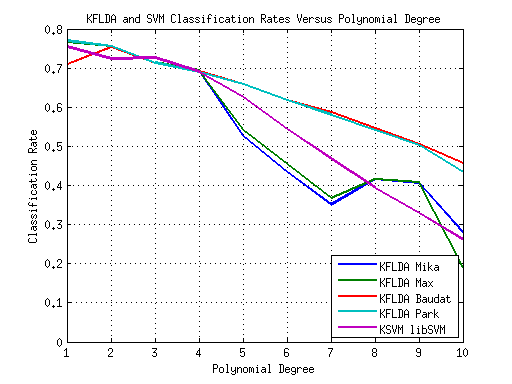
\includegraphics[width=3.3in]{../images/poly_kernel_optimize_2.png}
\caption{Searching For Best Polynomial Degree from 1 to 10. Classification Rates Versus Polynomial Degree. KFLDA using Euclidean distance.}
\label{fig:poly_kernel_eu}
\end{figure}

\par For the tangent hyperbolic sigmoid kernel we precede as in the polynomial case and set the parameter of \(c=0\) and then vary the amplitude \(gamma\) from \(0.01\) to \(1\). These limits were found empirically to give non-constant results and after \(1\) the classification rate was constant. This is not unexpected given the shape of the sigmoid function. You can see from the graph in \ref{fig:sig_kernel_eu} that the lower number give better results. We chose \(\gamma=0.01\) when using this kernel. Also, notice the SVM and Baudat implementations skew sharply after the origin. For Baudat, this is due to the fact that we are doing a Eigenvalue decomposition on the Gram matrix which is not of full rank and we assume the same for the SVM.

\begin{figure}[!h]
\centering
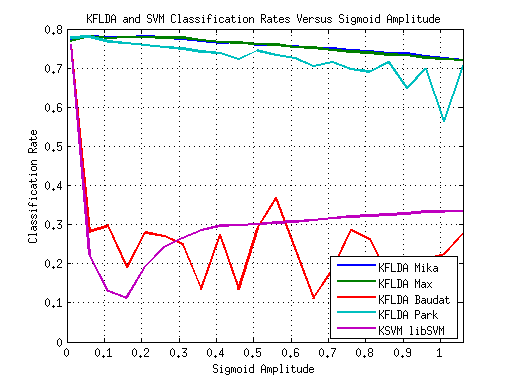
\includegraphics[width=3.3in]{../images/sig_kernel_optimize_2.png}
\caption{Searching For Best Sigmoid Amplitude 0.01 to 1. Classification Rates Versus Amplitude. KFLDA using Euclidean distance.}
\label{fig:sig_kernel_eu}
\end{figure}

\par For the RBF kernel we precede as before and varied the RBF variance \(\sigma\) from \(1\) to \(10\). After examining figure \ref{fig:rbf_kernel_eu} we see the best classification rate was chosen at \(\sigma=3\). Also, note the consistency of the result among the different algorithms. This is attributed to the fact that the Gram matrix will have full rank in most cases because the RBF of a vector with itself will be \(e^0 = 1\).

\begin{figure}[!h]
\centering
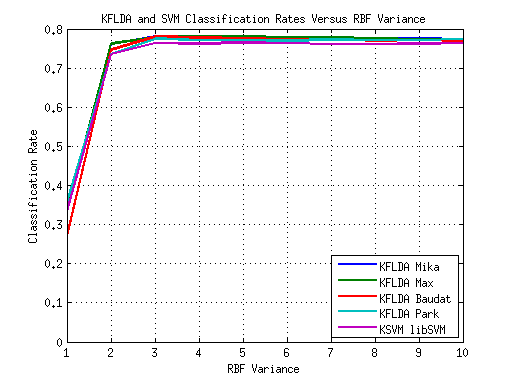
\includegraphics[width=3.3in]{../images/rbf_kernel_optimize_2.png}
\caption{Searching For Best RBF Variance from 1 to 10. Classification Rates Versus Variance. KFLDA using Euclidean distance.}
\label{fig:rbf_kernel_eu}
\end{figure}

\section{Algorithm Performance}
\par We evaluated the classifiers over a range of data set sizes. These subsets were chosen by randomly selecting a percentage of training samples from each class. Then the classification rate was computed by classifying all of observations in \(\Delta\). You can see the performance of the classifiers in figures \ref{fig:poly_size_eu}, \ref{fig:sig_size_eu} and \ref{fig:rbf_size_eu}. Among all the algorithms and data sizes it appears that KFLDA outperformed KSVM. Also, all the kernel methods outperformed the non-kernel FLDA and SVM when the amount of training data was low and using the RBF and polynomial kernels. The sigmoid kernel performed worst of all three for KSVM, but best overall for KFLDA. We computed the same curves using the Mahalanobis distance, and found the same trends. These graphs are not included here due to space.

\begin{figure}[!h]
\centering
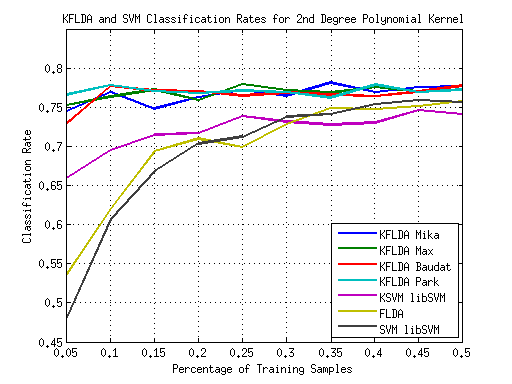
\includegraphics[width=3.3in]{../images/poly_size_3.png}
\caption{Polynomial Kernel \(degree = d = 2\). KFLDA using Euclidean distance. Classification Rates Versus Class Subset Size as Percentage of Each Class.}
\label{fig:poly_size_eu}
\end{figure}

\begin{figure}[!h]
\centering
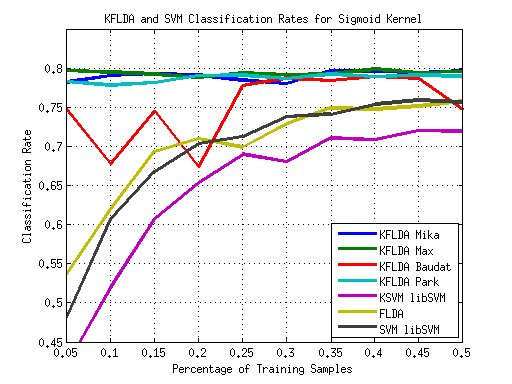
\includegraphics[width=3.3in]{../images/sig_size_3.png}
\caption{Sigmoid kernel \(Amplitude = \gamma = 0.01\). KFLDA using Euclidean distance. Classification Rates Versus Class Subset Size as Percentage of Each Class.}
\label{fig:sig_size_eu}
\end{figure}

\begin{figure}[!h]
\centering
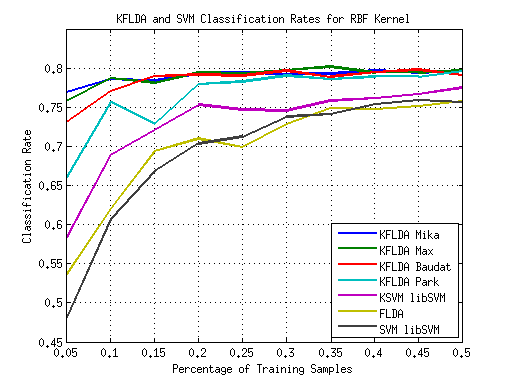
\includegraphics[width=3.3in]{../images/rbf_size_3.png}
\caption{RBF kernel \(Variance = \sigma = 3\). KFLDA using Euclidean distance. Classification Rates Versus Class Subset Size as Percentage of Each Class.}
\label{fig:rbf_size_eu}
\end{figure}

\section{SVM Investigations, One Sample and Multi-Class}
\par We also investigated some of the limits of SVM using only five support vectors, one training sample from each class. For each kernel, we choose five random support vectors and then trained and classified all of \(\Delta\) 100 times. The results are shown in figure \ref{fig:libsvm_1sample}. We ran LibSVM with each kernel using the optimized parameters we found when optimize for the entire data set \(\Delta\) and found the classification rate was around 20\%. However, if we re-optimized the kernel parameter search using just five support vectors we arrive at the classification rates in columns 5, 6 and 7 which vary from 35\% to 43\%. This data strongly suggests that you need to retrain your classifier and optimize your kernel parameters for each training data set size.

\begin{figure}[!h]
\centering
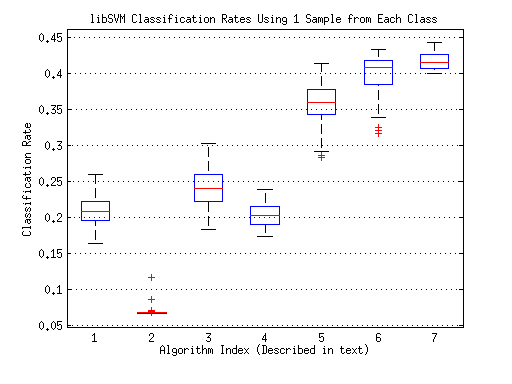
\includegraphics[width=3.3in]{../images/libSVM_1Sample.png}
\caption{LibSVM using 1 sample from each class. (1) No kernel, (2) Polynomial \(\gamma = 1, c=0, d=2\), (3) Sigmoid \(\gamma=0.01, c=0\), (4) RBF \(\sigma=3\), (5) Polynomial \(\gamma=1, c=0, d=\sqrt{2}\), (6) Sigmoid \(\gamma=0.0331, c=0\), (7) RBF \(sigma=0.15\)}
\label{fig:libsvm_1sample}
\end{figure}

\par During our testing it became known that LibSVM does a one-to-one decomposition of the multi-class problem. We wanted to assess if a true multi-class approach could do better. Therefore, we found MCSVM by Koby Crammer \cite{mcsvm} and MSVM-Pack by Lauer and Guermeur \cite{msvmpack}. We ran MCSVM for all three kernels at the optimized parameters using all of \(\Delta\) for training and testing as before. The classification rates are shown in figure \ref{fig:msvm_kernel}. The figure shows that RBF does the best job, and sigmoid and polynomial do not perform well. We attempted to use the MSVM-Pack implementation, but found the run time to be prohibitive. From runs of very small data sets, we found anecdotal data that suggests that MSVM-Pack performs as well as MCSVM, but more work would be need to substantiate that claim fully.

\begin{figure}[!h]
\centering
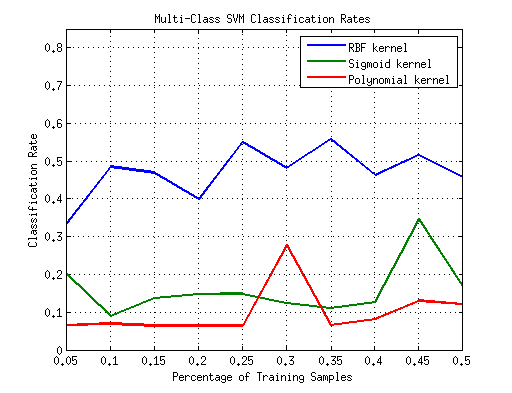
\includegraphics[width=3.3in]{../images/msvm_kernel_rates.png}
\caption{Multi-Class SVM using Crammer \cite{mcsvm} for all kernels.}
\label{fig:msvm_kernel}
\end{figure}

\section{Classifications Rates per Class}
\par The above analysis only considers the overall classification rate for each data subset, algorithm and kernel. We also investigated the individual classification rates to see if one class was dominating the others. Figures \ref{fig:indiv_eu} and \ref{fig:indiv_svm} show the individual class classification rates for KFLDA and SVM using the RBF and differing data sets sizes. Both graphs show that classes one and five are dominating the correct classification rate. Due to the linear nature of the data, classes one and five only share one hyperplane between itself and the remaining classes. While classes two, three and four share two separating hyperplanes with the remaining classes.

\begin{figure}[!h]
\centering
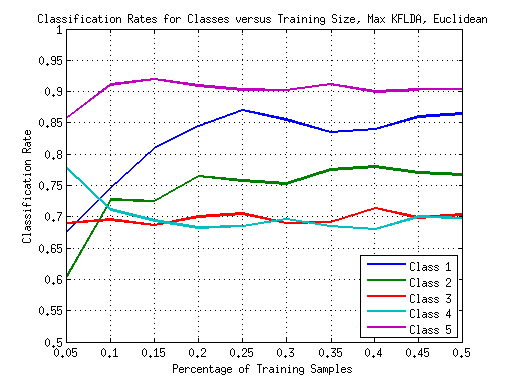
\includegraphics[width=3.3in]{../images/individual_class_euclid.png}
\caption{Individual Classification Rates for each Class using RBF kernel \(\sigma=3\), KFLDA by Max \cite{max} and Euclidean Distance Metric.}
\label{fig:indiv_eu}
\end{figure}

\begin{figure}[!h]
\centering
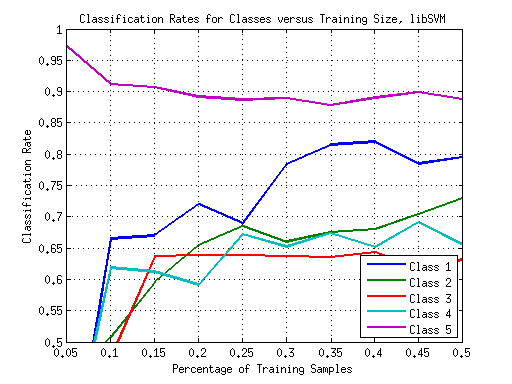
\includegraphics[width=3.3in]{../images/individual_class_svm.png}
\caption{Individual Classification Rates for each Class using RBF kernel \(\sigma=3\), libSVM \cite{libsvm}.}
\label{fig:indiv_svm}
\end{figure}

\section{Algorithm Run Time Performance}
\par We found the run times of the classifiers varied depending on the implementation. For example, LibSVM is written in C code while all the KFLDA implementations were done in Matlab. The run times versus data size are plotted in figure \ref{fig:alg_times}. You can see that FLDA and SVM had similar run times. This is interesting because FLDA was computed using Matlab code. This implies that the dominating run time component for the KFLDA implementations is the Gram matrix computation and Eigenvalue decompositions and SVD. Notice that the Park and Baudat had the worst run times but also do not require a regularization constant. Also, notice that Mika and Max has similar run times and similar classification performance. Finally, the run time of the Gram matrix computation was evaluated and found, as expected, the RBF was higher than the sigmoid and polynomial was the lowest.

\begin{figure}[!h]
\centering
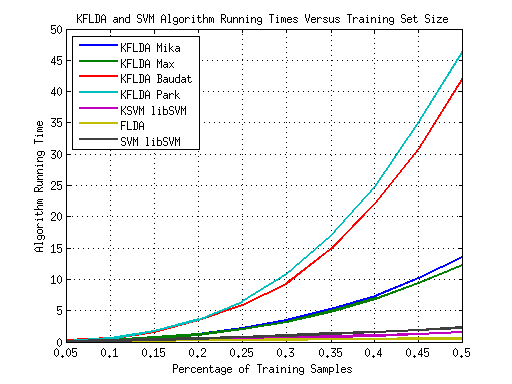
\includegraphics[width=3.3in]{../images/alg_times.png}
\caption{Algorithm run times for KFLDA Algorithms, libSVM and FLDA versus Class Subset Size as Percentage of Each Class.}
\label{fig:alg_times}
\end{figure}

\section{Conclusion}
\par In this study, we investigated the improvements that could be achieved using a kernel based approach to SVM and FLDA classifiers. We found that using a kernel allows a better classification rate with fewer samples, but does not improve overall classification rate when FLDA or SVM has sufficient samples. Also that optimizing kernel parameters for each training data set size is a good practice.
\par The Mika, Max, Baudat and Park KFLDA did best overall and the sigmoid kernel did the best using KFLDA, but the worst using KSVM. The Baudat and Park KFLDA do not require a regularization, but have high run time complexities. We were also surprised by how well that KSVM does using only one support vector per class.
\par Even though we did not include the Mahalanobis graphs in the paper, we discovered Mahalanobis distance did not do as well as Euclidean distance. However, the other distance metric did show the same trends overall. To investigate this further, we did a run using a data set using an equal number observations from each class (i.e. we made the priors equal). This shows the same trend that the Mahalanobis distance still did not do as well. We concluded that the assumption of a Gaussian class conditional probability model may be flawed when using a kernel. However, the Gaussian model is robust to non-Gaussian characteristics, so this may imply that the data is highly skewed. More work will need to be done to verify this finding.

% References section
\bibliographystyle{plain}
\bibliography{./references}

% Biography
\begin{IEEEbiographynophoto}{Bernard Lampe}
(M'09) became an IEEE Member (M) in 2009 and received his bachelors of science degree from The University of Michigan in Ann Arbor, Michigan, USA in 2009. Mr. Lampe is also a member of the American Society for Computing Machines (ACM) since 2009.
\end{IEEEbiographynophoto}

% End document
\end{document}

